\documentclass[hidelinks, 11pt, a4paper]{article}[24.03.2023]
    %hidelinks pouzivame s kombinaci hyperref, aby reference nebyly vyznaceny a nebiky tak moc do oci
    \usepackage[left=2cm, top=3cm, text={17cm, 24cm}]{geometry}
    \usepackage[utf8]{inputenc}
    \usepackage[czech]{babel}
    \usepackage[IL2]{fontenc}
    \usepackage[vlined,linesnumbered,noline,longend,ruled]{algorithm2e}
    \usepackage{times}
    \usepackage{multirow} 
    \usepackage{hyperref}
    \usepackage{picture}
    \usepackage{graphics}
    \usepackage{pdflscape}
    
    


\begin{document}

    \begin{titlepage}
        \begin{center}
            {\Huge \textsc{Vysoké učení technické v~Brně}\\[0.5em]}
            {\huge \textsc{Fakuklta informačních technologií}}
            \vspace{\stretch{0.382}}

            {\LARGE Typografie a publikování -- 3.projekt\\[0.4em]}
            {\huge Tabulky a obrázky}

            \vspace{\stretch{0.618}}
            {\Large \today \hfill Roman Machala}

        \end{center}
    \end{titlepage}

\section{Úvodní strana}
    Název práce umístěte do zlatého řezu a nezapomeňte uvést \uv{dnešní} (today) datum a vaše jméno a příjmení.
    
\section{Tabulky}
    Pro sázení tabulek můžeme použít buď prostředí\; \verb|tabbing|\; nebo prostředí\; \verb|tabular|. 
    \subsection[tabbing]{Prostředí \texttt{tabbing}}
        Při použití\; \verb|tabbing|\; vypadá tabulka následovně:
        \begin{tabbing}
            %Vuyžijeme nejdelších slov na každém řádku k nastavení zarážek
            Vodní melouny\quad \= 25,90\quad \= Množství \kill
            \textbf{Ovoce} \> \textbf{Cena} \> \textbf{Množství} \\
            Jablka \> 25,90 \> 3 kg  \\
            Hrušky \> 27,40 \> 2,5 kg  \\
            Vodní meloun \> 35,-- \> 1 kus
        \end{tabbing}
        Toto prostředí se dá teké použít pro sázení algoritmů, ovšem vhodnější je použít prostředí\; \verb|algorithm|\;~nebo \verb|algorithm2e|\; (viz sekce \ref{Algoritmy}).

        \subsection[tabualar]{Prostředí \texttt{tabular}}
            Další možnost, jak vytvořit tabulku, je použít prostředí\; \verb|tabular|. Tabulky pak budou vypadat takto\footnote[1]{Kdyby byl problém s\; \texttt{cline}, zkuste se podívat třeba sem: \href{http://www.abclinuxu.cz/tex/poradna/show/325037}{http://www.abclinuxu.cz/tex/poradna/show/325037}.}:
            \begin{table}[h]
            \catcode`\-=12  %Vloženi catcode,nalezeno na https://www.abclinuxu.cz/tex/poradna/show/325037, řešení pro \cline 
                \begin{center}
                    \begin{tabular}[t]{| c | c | c |}\hline
                        & \multicolumn{2}{ |c| }{\textbf{Cena}} \\ \cline{2-3}
                        \textbf{Měna} & \textbf{nákup} & \textbf{prodej} \\ \hline
                        EUR & 22,705 & 25,242 \\
                        GBP & 25,931 & 28,828 \\
                        USD & 21,347 & 23,732 \\\hline
                    \end{tabular}
                    \caption{Tabulka kurzů k~dnešnímu dni} 
                    \label{Kurzy}
                \end{center}
            \end{table}
        \begin{center}
            \begin{table}[h]
                %catcode prilozen z duvodu problemu s prikazem cline
                \catcode`\-=12
                %Tabulka cislo 1
                    \begin{tabular}{| c | c |} \hline
                        $A$ & $\neg A$ \\ \hline
                        \textbf{P} & N \\ \hline
                        \textbf{O} & O~\\ \hline
                        \textbf{X} & X \\ \hline
                        \textbf{N} & P \\ \hline
                    \end{tabular}
                %Tabulka cislo 2
                    \begin{tabular}{| c | c | c | c | c | c |} \hline
                        \multicolumn{2}{ | c | }{\multirow{2}{*}{A $\land$ B}} & \multicolumn{4}{ | c | }{$B$} \\ \cline{3-6}
                        \multicolumn{2}{ | c | }{} & \textbf{P} & \textbf{O} & \textbf{X} & \textbf{N} \\ \hline
                        \multirow{4}{*}{A} & \textbf{P} & P & O~& X & N \\ \cline{2-6}
                        & \textbf{O} & O~& O~& N & N \\ \cline{2-6}
                        & \textbf{X} & X & N & X & N \\ \cline{2-6}
                        & \textbf{N} & N & N & N & N \\ \hline
                    \end{tabular}
                %Tabulka cislo 3
                    \begin{tabular}{| c | c | c | c | c | c |} \hline
                        \multicolumn{2}{ | c | }{\multirow{2}{*}{A $\lor$ B}} & \multicolumn{4}{ | c | }{$B$} \\ \cline{3-6}
                        \multicolumn{2}{ | c | }{} & \textbf{P} & \textbf{O} & \textbf{X} & \textbf{N} \\ \hline
                        \multirow{4}{*}{A} & \textbf{P} & P & P & P & P \\ \cline{2-6}
                        & \textbf{O} & P & O~& P & O~\\ \cline{2-6}
                        & \textbf{X} & P & P & X & X \\ \cline{2-6}
                        & \textbf{N} & P & O~& X & N \\ \hline
                    \end{tabular}
                %Tabulka cislo 4
                    \begin{tabular}{| c | c | c | c | c | c |} \hline
                        \multicolumn{2}{ | c | }{\multirow{2}{*}{A $\rightarrow$ B}} & \multicolumn{4}{ | c | }{$B$} \\ \cline{3-6}
                        \multicolumn{2}{ | c | }{} & \textbf{P} & \textbf{O} & \textbf{X} & \textbf{N} \\ \hline
                        \multirow{4}{*}{A} & \textbf{P} & P & O~& X & N \\ \cline{2-6}
                        & \textbf{O} & P & O~& P & O~\\ \cline{2-6}
                        & \textbf{X} & P & P & X & X \\ \cline{2-6}
                        & \textbf{N} & P & P & P & P \\ \hline
                    \end{tabular}
                \caption{Protože Kleeneho trojhodnotová logika už je \uv{zastaralá}, uvádíme si zde příklad čtyřhodnotové logiky}\label{Logika}
            \end{table}
        \end{center}
    
        \section{Algoritmy}
            \label{Algoritmy}
            Pokud budeme chtít vysázet algoritmus, můžeme použít prostředí\; \verb|algorithm|
            \footnote[2]{Pro nápovědu, jak zacházet s~prosředím \texttt{algorithm}, můžeme zkusit 
            tuhle stránku: 
            
            \href{http://ftp.cstug.cz/pub/tex/CTAN/macros/latex/contrib/algorithms/algorithms.pdf}{http://ftp.cstug.cz/pub/tex/CTAN/macros/latex/contrib/algorithms/algorithms.pdf}.}\; 
            nebo \; \verb|algorithm2e|\footnote[3]{Pro\; \texttt{algorithm2e}\; zase tuhle:\;\href{http://ftp.cstug.cz/pub/tex/CTAN/macros/latex/contrib/algorithm2e/doc/algorithm2e.pdf}{http://ftp.cstug.cz/pub/tex/CTAN/macros/latex/contrib/algorithm2e/doc/algorithm2e.pdf}.}.
            Příklad použití prostředí \; \verb|algorithm2e| \; viz Algoritmus \ref{Alg1}.
            \renewcommand{\algorithmcfname}{Algoritmus}%Alternativa, pokud nedavame do prembule u \usepackage{algorithm2e} moznost czech
      
    \SetNlSty{}{}{:} %Nastavime za cislovanim kazdeho radku ":"
    \begin{algorithm}[H]\label{Alg1}
        \caption{\textsc{Fast}SLAM}
        \Indm
        \KwIn{$(X_{t -1}, u_t, z_t)$}
        \KwOut{$X_t$}
        \Indp\Indpp
        $\overline{X_t} = X_t = 0$ \\
        \For{$k = 1 $ \normalfont{to} $M$}{$x_{t}^{\left[k\right]} = \textit{sample\_motion\_model}(u_t,x_{t-1}^{\left[k\right]})$ \\
        $\omega_t^{\left[k\right]} = \textit{measurement\_model}(z_t,x_t^{\left[k\right]},m_{t-1})$ \\
        $m_t^{\left[k\right]} = updated\_occupancy\_grid(z_t,x_t^{\left[k\right]},m_{t-1}^{\left[k\right]})$ \\
        $\overline{X_t} = \overline{X_t} + \langle x_x^{\left[m\right]},\omega_t^{\left[m\right]}\rangle$}
        \For{$k = 1$\ {\upshape to} $M$}
            {draw $i$ with probability $\approx \omega_t^{\left[i\right]}$ \\
            add $\langle x_x^{\left[k\right]},m_t^{\left[k\right]}\rangle$ to $X_t$}
        \KwRet{$X_t$}
    \end{algorithm}

    \section{Obrázky}
        Do našich článků můžeme samozřejmě vkládat obrázky.
        Pokud je obrázkem fotografie, můžeme klidně použít bitmapový soubor. Pokud by to ale mělo být nějaké schéma nebo něco podobného,
        je dobrým zvykem takovýto obrázek vytvořit vektorově.
    \begin{figure}[!ht]
            \hfill\scalebox{0.45}{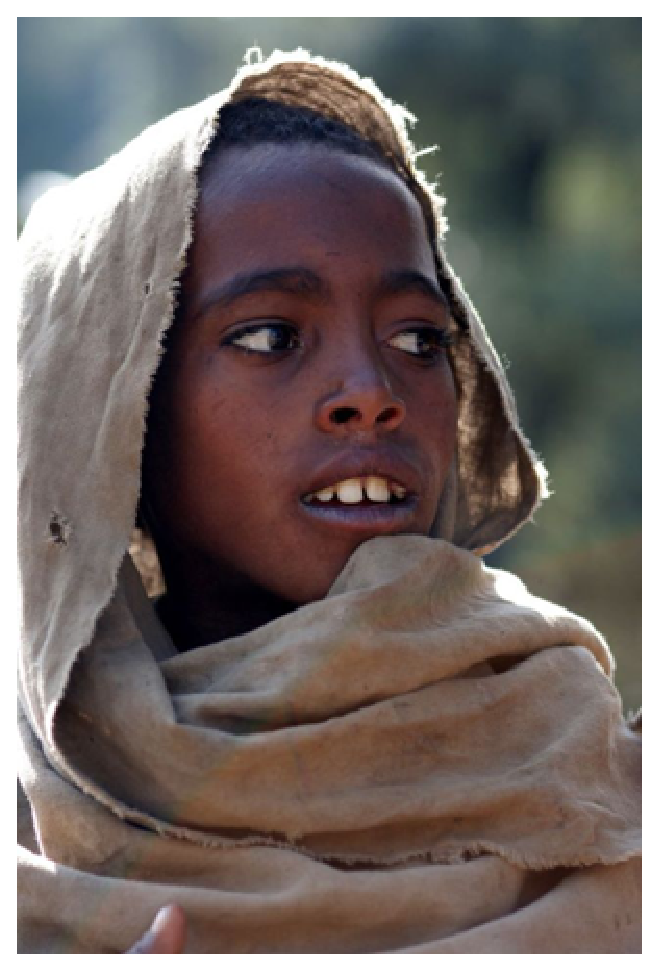
\includegraphics{etiopan.eps}}
            \reflectbox{\scalebox{0.45}{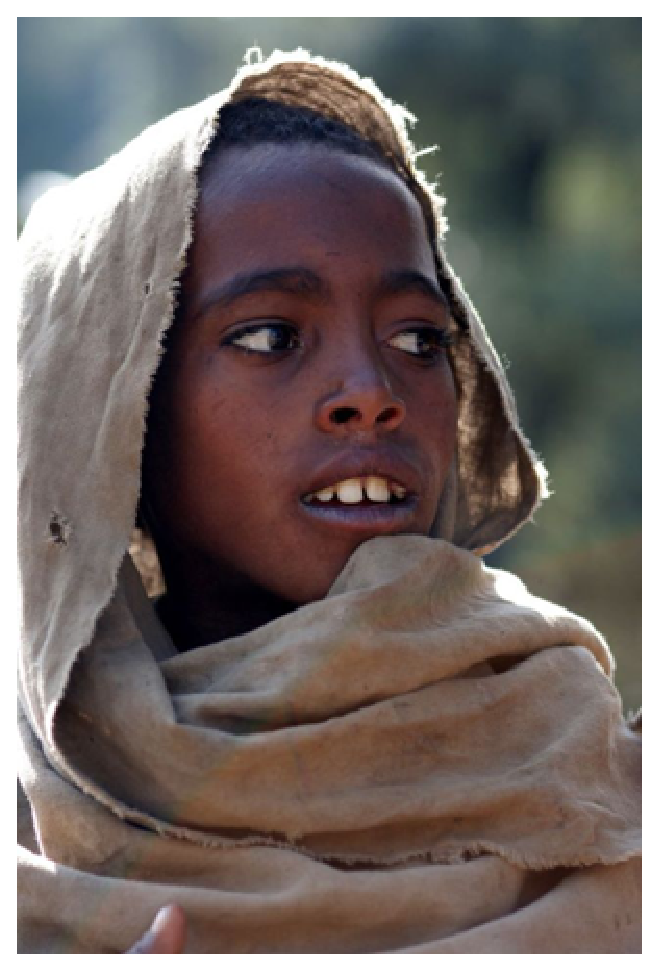
\includegraphics{etiopan.eps}}}\hspace*{\fill}
            \caption{Malý Etiopiánek a jeho bratříček}\label{Obr1}
    \end{figure}

	\pagebreak
    Rozdíl mezi vektorovým\dots
    \begin{figure}[!ht]
        \hfill\scalebox{0.45}{
\includegraphics{oniisan.eps}}\hspace*{\fill}
        \caption{Vektrorový obrázek}\label{Obr2}
    \end{figure}

    \dots a bitmapovým obrázkem

    \begin{figure}[!ht]
        \hfill\scalebox{0.6}{
\includegraphics{oniisan2.eps}}\hspace*{\fill}
        \caption{Bitmapový obrázek}\label{Obr3}
    \end{figure}

    se projeví například při zvětšení.

    Odkazy (nejen ty) na obrázky \ref{Obr1},\,\ref{Obr2} a \ref{Obr3} a na tabulky \ref{Kurzy} a \ref{Logika} a také na algoritmus \ref{Alg1} jsou udělány pomocí křížových odkazů.
    Pak je ovšem potřeba zdrojový soubor přeložit dvakrát.

    Vektorové obrázky lze vytvořit i přímo v~\LaTeX\textnormal{u}, například pomocí prostředí\; \verb|picture|. 


    \setlength{\unitlength}{1cm}
        %Nastavime zakladni velikosti pro kresleni v prostredi picture jako nasobky 1 cm misto 1 pt
        
    \begin{landscape}
    \begin{figure}[!ht]
    \begin{center}
            \begin{picture}(17, 12)
                %Vykresleni hlavniho obrysu se schody
                \put(0,0){\framebox(17, 10)}
                \put(15.5, 8.5){\circle{1.25}}
                \put(3, 1.5){\thicklines\framebox(11, 4)}
                \multiput(7.875,1.25)(0, -0.25){3}{\framebox(1.25, 0.25)}
                \multiput(7.75, 1.5)(0.75, 0){2}{\framebox(0.75, 1.5)}
                %Vykresleni dveri a detaily k nim
                \multiput(7.875, 1.675)(0.75, 0){2}{\framebox(0.5, 1.25)}
                \multiput(7.875, 1.675)(0, 0.25){5}{\line(1,0){0.5}}
                \multiput(8.625, 1.675)(0, 0.25){5}{\line(1,0){0.5}}
                %Kresleni balkonu nad dvermi 
                \put(7, 3){\framebox(3,0.1)}
                \multiput(7, 3.1)(0.485, 0){6}{\framebox(0.1, 0.2)}
                \put(9.9, 3.1){\framebox(0.1, 0.2)}
                \put(6.8, 3.3){\framebox(3.4, 0.1)}
                %Kresleni piliru  
                \multiput(7.1, 1.6)(2.5,0){2}{\framebox(0.3, 1.3)}
                \multiput(7, 1.5)(0, 1.4){2}{\framebox(0.5, 0.1)}
                \multiput(9.5, 1.5)(0, 1.4){2}{\framebox(0.5, 0.1)}
                
                %Kresleni oken ve spodnim patre
                \multiput(4.5, 2)(7, 0){2}{\framebox(1, 1)}
                \multiput(4, 2)(1.5, 0){2}{\framebox(0.5, 1)}
                \multiput(11, 2)(1.5, 0){2}{\framebox(0.5, 1)}
                \multiput(4, 2)(0, 0.2){5}{\line(1, 0){0.5}}
                \multiput(5.5, 2)(0, 0.2){5}{\line(1, 0){0.5}}
                \multiput(11, 2)(0, 0.2){5}{\line(1, 0){0.5}}
                \multiput(12.5, 2)(0, 0.2){5}{\line(1, 0){0.5}}
                \put(5, 2){\line(0,1){1}}
                \put(4.5, 2.5){\line(1,0){1}}
                \put(12, 2){\line(0,1){1}}
                \put(11.5, 2.5){\line(1,0){1}}

                %Dokonceni balkonu
                %\put(7.9, 3){\framebox(1.2, 1.5)}
                \put(7.9, 4.5){\line(1,0){1.2}}
                \put(7.9, 3.4){\line(0,1){1.1}}
                \put(9.1, 3.4){\line(0,1){1.1}}
                \put(7.9, 3.1){\line(0,1){0.2}}
                \put(9.1, 3.1){\line(0,1){0.2}}
                \put(8.5, 3.4){\line(0,1){1.1}}
                \multiput(8.025, 3.5)(0.6,0){2}{\framebox(0.35, 0.8)}
                
                %Vykresleni oken ve druhem patre
                \multiput(4, 3.8)(6.9, 0){2}{\framebox(2.1,1)}
                \multiput(4.7, 3.8)(0.7,0){2}{\line(0, 1){1}}
                \multiput(11.6, 3.8)(0.7,0){2}{\line(0, 1){1}}
                \put(4, 4.3){\line(1, 0){2.1}}
                \put(10.9, 4.3){\line(1, 0){2.1}}

                %Vykresleni strechy
                \put(3, 5.5){\line(1, 1){2}}
                \put(14, 5.5){\line(-1, 1){2}}
                \put(5, 7.5){\line(1, 0){1}}
                \put(12, 7.5){\line(-1, 0){0.5}}
                \put(11, 7.5){\framebox(0.5,1)}
                \multiput(11, 7.5)(0, 0.2){5}{\line(1, 0){0.5}}
                \put(11.25, 7.5){\line(0, 1){1}}
                \put(6, 7.5){\line(1,0){5}}
            \end{picture}
        \caption{Vektorový obrázek moderního bydlení vhodného pro 21. století. (Buď to vytvořte stejný obrázek, anebo nakreslete pomocí\; \texttt{picture}\; váš vlastní domov.)}
    \end{center}
    \end{figure}
    \end{landscape}


    
\end{document} 
